% Options for packages loaded elsewhere
\PassOptionsToPackage{unicode}{hyperref}
\PassOptionsToPackage{hyphens}{url}
\PassOptionsToPackage{dvipsnames,svgnames,x11names}{xcolor}
%
\documentclass[
]{jds}

\usepackage{amsmath,amssymb}
\usepackage{iftex}
\ifPDFTeX
  \usepackage[T1]{fontenc}
  \usepackage[utf8]{inputenc}
  \usepackage{textcomp} % provide euro and other symbols
\else % if luatex or xetex
  \usepackage{unicode-math}
  \defaultfontfeatures{Scale=MatchLowercase}
  \defaultfontfeatures[\rmfamily]{Ligatures=TeX,Scale=1}
\fi
\usepackage{lmodern}
\ifPDFTeX\else  
    % xetex/luatex font selection
\fi
% Use upquote if available, for straight quotes in verbatim environments
\IfFileExists{upquote.sty}{\usepackage{upquote}}{}
\IfFileExists{microtype.sty}{% use microtype if available
  \usepackage[]{microtype}
  \UseMicrotypeSet[protrusion]{basicmath} % disable protrusion for tt fonts
}{}
\makeatletter
\@ifundefined{KOMAClassName}{% if non-KOMA class
  \IfFileExists{parskip.sty}{%
    \usepackage{parskip}
  }{% else
    \setlength{\parindent}{0pt}
    \setlength{\parskip}{6pt plus 2pt minus 1pt}}
}{% if KOMA class
  \KOMAoptions{parskip=half}}
\makeatother
\usepackage{xcolor}
\setlength{\emergencystretch}{3em} % prevent overfull lines
\setcounter{secnumdepth}{-\maxdimen} % remove section numbering
% Make \paragraph and \subparagraph free-standing
\makeatletter
\ifx\paragraph\undefined\else
  \let\oldparagraph\paragraph
  \renewcommand{\paragraph}{
    \@ifstar
      \xxxParagraphStar
      \xxxParagraphNoStar
  }
  \newcommand{\xxxParagraphStar}[1]{\oldparagraph*{#1}\mbox{}}
  \newcommand{\xxxParagraphNoStar}[1]{\oldparagraph{#1}\mbox{}}
\fi
\ifx\subparagraph\undefined\else
  \let\oldsubparagraph\subparagraph
  \renewcommand{\subparagraph}{
    \@ifstar
      \xxxSubParagraphStar
      \xxxSubParagraphNoStar
  }
  \newcommand{\xxxSubParagraphStar}[1]{\oldsubparagraph*{#1}\mbox{}}
  \newcommand{\xxxSubParagraphNoStar}[1]{\oldsubparagraph{#1}\mbox{}}
\fi
\makeatother


\providecommand{\tightlist}{%
  \setlength{\itemsep}{0pt}\setlength{\parskip}{0pt}}\usepackage{longtable,booktabs,array}
\usepackage{calc} % for calculating minipage widths
% Correct order of tables after \paragraph or \subparagraph
\usepackage{etoolbox}
\makeatletter
\patchcmd\longtable{\par}{\if@noskipsec\mbox{}\fi\par}{}{}
\makeatother
% Allow footnotes in longtable head/foot
\IfFileExists{footnotehyper.sty}{\usepackage{footnotehyper}}{\usepackage{footnote}}
\makesavenoteenv{longtable}
\usepackage{graphicx}
\makeatletter
\def\maxwidth{\ifdim\Gin@nat@width>\linewidth\linewidth\else\Gin@nat@width\fi}
\def\maxheight{\ifdim\Gin@nat@height>\textheight\textheight\else\Gin@nat@height\fi}
\makeatother
% Scale images if necessary, so that they will not overflow the page
% margins by default, and it is still possible to overwrite the defaults
% using explicit options in \includegraphics[width, height, ...]{}
\setkeys{Gin}{width=\maxwidth,height=\maxheight,keepaspectratio}
% Set default figure placement to htbp
\makeatletter
\def\fps@figure{htbp}
\makeatother

\makeatletter
\@ifpackageloaded{caption}{}{\usepackage{caption}}
\AtBeginDocument{%
\ifdefined\contentsname
  \renewcommand*\contentsname{Table of contents}
\else
  \newcommand\contentsname{Table of contents}
\fi
\ifdefined\listfigurename
  \renewcommand*\listfigurename{List of Figures}
\else
  \newcommand\listfigurename{List of Figures}
\fi
\ifdefined\listtablename
  \renewcommand*\listtablename{List of Tables}
\else
  \newcommand\listtablename{List of Tables}
\fi
\ifdefined\figurename
  \renewcommand*\figurename{Figure}
\else
  \newcommand\figurename{Figure}
\fi
\ifdefined\tablename
  \renewcommand*\tablename{Table}
\else
  \newcommand\tablename{Table}
\fi
}
\@ifpackageloaded{float}{}{\usepackage{float}}
\floatstyle{ruled}
\@ifundefined{c@chapter}{\newfloat{codelisting}{h}{lop}}{\newfloat{codelisting}{h}{lop}[chapter]}
\floatname{codelisting}{Listing}
\newcommand*\listoflistings{\listof{codelisting}{List of Listings}}
\makeatother
\makeatletter
\makeatother
\makeatletter
\@ifpackageloaded{caption}{}{\usepackage{caption}}
\@ifpackageloaded{subcaption}{}{\usepackage{subcaption}}
\makeatother

\ifLuaTeX
  \usepackage{selnolig}  % disable illegal ligatures
\fi
\usepackage[]{natbib}
\bibliographystyle{plainnat}
\usepackage{bookmark}

\IfFileExists{xurl.sty}{\usepackage{xurl}}{} % add URL line breaks if available
\urlstyle{same} % disable monospaced font for URLs
\hypersetup{
  pdftitle={My wonderful paper},
  colorlinks=true,
  linkcolor={blue},
  filecolor={Maroon},
  citecolor={Blue},
  urlcolor={Blue},
  pdfcreator={LaTeX via pandoc}}


\title{My wonderful paper}
\author{}
\date{}

\begin{document}
\maketitle
\begin{abstract}
This is the abstract
\end{abstract}

\renewcommand*\contentsname{Table of contents}
{
\hypersetup{linkcolor=}
\setcounter{tocdepth}{3}
\tableofcontents
}

\newpage

\section{Introduction}\label{introduction}

{[}background - In a data analysis workflow{]}

In a data analysis workflow -\textgreater{} going back to diagnose the
descripency between the expectation and the result is often
time-consuming and challenging.

For consumers of data analysis, it is often difficult to evaluate the
analysis outcome. Not always have the script to run, even difficult when
different expectations are held.

We propose here a concept called analysis plan to make the expectation
of the analysis process explicit. It can help to guide the analysis
process, to communicate and compare the analysis process to others, and
to evaluate the analysis process. (think more closer here how our
approach help to solve the problem)

For expert analysts, the expectation of the analysis process is often
implicit. They may have a mental model of the analysis process and the
expected results. However, for non-expert analysts, the expectation of
the analysis process may not be clear. They may not know what to expect
from the analysis process, or what to look for when an analysis process
fails the expectation. An analysis plan can help to make the expectation
of the analysis process explicit. It can help to guide the analysis
process, to communicate and compare the analysis process to others, and
to evaluate the analysis process.

In this paper, a concept called analysis plan is proposed to describe
the logical structure of a data analysis. An analysis plan is a set of
analysis steps plus their expected outcomes. It is a formal
representation of the analysis process and can be used to guide the
analysis process, to communicate and compare the analysis process to
others, and to evaluate the analysis process. The concept of analysis
plan is illustrated with examples. The implications of the concept for
data analysis practice is discussed.

The analysis plan described in this paper should be differentiated from
the pre-specifies analysis plan document often used in biostatistics to
specifies the hypothesis, data collection mechanism, statistical
procedures etc of randomized experiments.

The rest of the paper is organized as follows: Section~\ref{sec-plan}
describes the concept of analysis plan in detail.
Section~\ref{sec-examples} provides examples of analysis plan {[}more
details{]}. (need another section here or before examples?)
Section~\ref{sec-conclusion} concludes the paper.

\section{Literature review}\label{literature-review}

\subsection{Diagnosing unexpected outcomes in data
analysis}\label{diagnosing-unexpected-outcomes-in-data-analysis}

\subsection{Unit tests}\label{unit-tests}

\subsection{Data quality checks}\label{data-quality-checks}

\section{Analysis plan}\label{sec-plan}

\subsection{Framing checks into unit
tests}\label{framing-checks-into-unit-tests}

Q: Whether we should formulate these concept with math notation?? A:
only if it helps

TODO: more about analysis plan itself here

TODO: what if the expectation is ``wrong''

The whole point being how can be build trust in other's analysis. Some
provides scripts to run the analysis but that's not enough. We need to
know what to expect from the analysis and that is often not explicitly
specified.

An analysis plan is a set of analysis steps combined with expectations.
Expectations represent our belief about certain aspects of the analysis,
independent of the analysis itself. It can be divided into two types:
\emph{outcome expectation} and \emph{plan expectation}. Outcome
expectation refers to what we anticipate from the main result of the
analysis based on prior knowledge. They shape how we interpret the
results and assess whether they are consistent with existing knowledge
or indicate the need for updates \citep{grolemund_cognitive_2014}. For
example, in public health, prior research shows the average increase in
mortality rate per unit increase in PM10 is about 0.50\%
\citep{liu2019ambient}. This serves as an expectation for similar future
studies. Plan expectations concern the intermediate steps within the
analysis rather than the final outcome. They serve as checkpoints to
detect deflection in the analysis process For example, we may expect
temporal data to be ordered with no gaps and duplicates, or expect that
temperature will be a significant covariate in the linear regression
model of PM10 on mortality.

(might be useful) Analysis plans can be constructed at various
granularities, at the highest level, one may only has a plan of the
specific method used for analysing data and the expected outcome. This
provides little guidance when a deviation from expectation occurs. At
the lowest level, one may have a plan for each data entry and every data
handling steps. This provides too much detail and may not be practical
in practice.

Experienced analysts often have implicit expectation about the outcome
and rely on a few ``directional signs'' to check when the outcome
deviate from those expectation. However, these expectations are rarely
made explicit within the analysis workflow. This makes it challenging
for consumers of the analysis to evaluate the results, since it becomes
difficult to disentangle whether discrepancies arise from differing
expectations or from the use of statistical technique, without running
the analysis themselves. Non-expert analysts, lacking prior knowledge or
instinct, may not have clear expectations of the results. This can lead
to reduced confidence of the analysis and makes it more difficult and
time-consuming to diagnose the cause of the deviation when the results
don't align with expectations. By explicitly formulating these
expectations, an analysis plan can guide the analysis process,
facilitate the communication and evaluate the validity of the results.

The expectations can be thought of as a set of unit tests used to
validate the results of data analysis. By specifying a range of values
for these tests, multiple versions of the dataset can be generated to
satisfy different sets of plan expectations. This allows us to present
what we called the ``result universe'' -- the complete set of possible
results that can be obtained from one data analysis process. By
visualizing the result universe, data analysis consumers can observe how
changes in expectations affect the results and the range of alternative
outcomes that could arise under different conditions. This enables them
to evaluate the outcomes based on their own plan expectations and gain a
broader perspective on how the actual results produced by analysts fit
within this spectrum of possibilities, promoting transparency and trust
in analysis.

Furthermore, by generating multiple versions of the data, we can emulate
various scenarios within the same context for students to exercise
judgement when conducting data analysis in a classroom setting.

\subsection{A toy example}\label{a-toy-example}

Let's think about a 5-day step count. You make a resolution to walk on
average 5000 steps a day (your expectation) and using an app to record
your step count. After 5 days, the app tells you've walked on average
8000 steps.

It is easy to come up with reasons why an 8000 average step is resulted
based on common sense:

\begin{enumerate}
\def\labelenumi{\arabic{enumi}.}
\tightlist
\item
  you may run a 10k on day 1, resulting a high step count on the day
  (outlier on the right).
\item
  you left your phone at home on day 3, resulting a zero or minimal step
  count on the day (outlier on the left).
\item
  you may realise the step count may increase since you were in a hiking
  trip in the last five days (average shift).
\end{enumerate}

Based on these reasons, you may devise a set of unit tests to check the
step count data, i.e.~check the maximum and minimum step count, check
the difference between each day.

\begin{itemize}
\tightlist
\item
  If the daily count looks like c(4000, 5000, 5500, 5500, 20000), the
  maximum check will flag the data for investigate the maximum. The
  difference between days test will also flag the data
\item
  If the daily count looks like c(20000, 20000, 20000, 20000, 20000),
  the maximum check will flag the data for investigate the maximum.
\end{itemize}

Some part of the space is impossible: c(0, 4000, 5000, 5500, 5500) is
flagged by the minimal tests but won't cause an average of 8000 average
step.

The statistical procedure of averaging 5 numbers ``around 5000'' to get
a mean of 5000 is \emph{consistent} meaning if all the numbers are
around 5000, we are guaranteed to get a mean around 5000. We could
devise 5 unit tests to check each number. Since you're more familiar
with your daily life, you may realise the step count may increase since
you were in a hiking trip in the last two days. This may prompt you to
check the step count.

In a data analysis, it is not practical to check every entry of the
data, a similar strategy of devising tests to check for

\begin{itemize}
\tightlist
\item
  The combination of unit tests are not unique
\item
  The unit tests provide guidance for diagnosing the results, but are
  not red flags: c(2000, 2000, 5000, 8000, 8000) will likely to fail the
  max diff test but receive a within expectation mean.
\end{itemize}

\section{Method}\label{method}

\subsection{A workflow to assess the quality of unit
tests}\label{a-workflow-to-assess-the-quality-of-unit-tests}

\begin{itemize}
\item
  multiple tests can be generated to diagnose different aspects of an
  analysis
\item
  good tests

  \begin{enumerate}
  \def\labelenumi{\arabic{enumi})}
  \tightlist
  \item
    are responsive to an unexpected result - accuracy,
  \item
    motivate actions of analysts to investigate the results. This points
    towards a smaller set of independent tests
  \end{enumerate}
\item
  Since both the plan/ outcome expectations can be phrased as unit
  tests, which output binary outcomes, consider using the plan
  expectations as predictors of the outcome expectations. This allows to
  generate the confusion matrix of predicting the outcome with the plan
  expectation.
\item
  For an analysis, ideally, good plan expectations should maximize the
  detection of unexpected outcomes while minimize the false positive
  discovery, which suggest the use of precision and recall (REF) for
  evaluating the performance of the plan expectations.

  \begin{itemize}
  \tightlist
  \item
    precision: the proportion of unexpected results (TP) out of all the
    predicted unexpected results (TP + FP)
  \item
    recall: the proportion of unexpected results (TP) out of all the
    actual unexpected results (TP + FN)
  \end{itemize}
\item
  A logic regression (ref) is used to model the relationship between the
  plan and outcome expectations. (justify the use of Logic regression)
\item
  on independence of the tests
\end{itemize}

\subsection{Toy example revisited}\label{toy-example-revisited}

\begin{itemize}
\item
  provide interpretation at different scenarios:

  \begin{enumerate}
  \def\labelenumi{\arabic{enumi})}
  \tightlist
  \item
    one test is flagged, the prediction is as expected:
  \item
    multiple tests are flagged, the prediction is unexpected,
  \item
    no test is flagged, the prediction is unexpected,
  \item
    no test is flagged, the prediction is as expected
  \end{enumerate}
\end{itemize}

\section{Applications}\label{sec-examples}

Three examples are presented to illustrate how the concept of analysis
plan can be applied to data analysis. {[}toy example{]}.
Section~\ref{sec-linear-reg} illustrates how constructing the result
universe in a linear regression model of PM10 on mortality can help
understand the impact of sample size, model specification, and variable
correlation structure on data analysis. {[}example three{]}

\subsection{Linear regression}\label{sec-linear-reg}

Consider a linear regression model to study the effect of PM10 on
mortality (provide context of using PM10 to study mortality). Analysts
may expect a significant (p-value \(\le\) 0.05) PM10 coefficient in the
linear model from the literature. This is the \emph{outcome
expectation}. There are multiple factors that can affect the outcome
expectation of linear regression, which here is called \emph{plan
expectation}, for example, 1) sample size, 2) model specification, and
3) correlation structure between variables. Adequate sample size is
required to achieve the desired power to detect the significance of PM10
on mortality. Temperature is often an important confounder to consider
in such study (add reference). From some domain knowledge, an analyst
may expect that the significance of PM10 coefficient can be attained by
adding temperature to the model. Analysts may also expect certain
correlation structure between PM10, temperature, and mortality, and the
distribution of each variable.

To build the result universe, datasets can be simulated to either meet
and fail these plan expectations, allowing the analysts to observe the
significance of PM10 coefficient. Here, sample sizes of 50, 100, 500,
and 1000 are considered. Two model specifications are included: 1)
linear model with PM10 as the only covariate
(\(\text{mortality} \sim \text{PM10}\)), 2) linear model with PM10 and
temperature as covariates
(\(\text{mortality} \sim \text{PM10} + \text{temp}\)). A grid-based
approach is used to simulate correlation structure. Reasonable ranges of
correlation between the three variables are
\(\text{cor}(\text{mortality}, \text{PM10}) \in [-0.01, 0]\),
\(\text{cor}(\text{mortality}, \text{temperature}) \in [-0.6, -0.2]\),
and \(\text{cor}(\text{PM10}, \text{temperature}) \in [0.2, 0.6]\).

\begin{itemize}
\item
  add a paragraph to describe the simulation process
\item
  add a fourth panel to describe the comparison of a right/ wrong
  expectation, i.e.~correlation on PM10 and mortality
\end{itemize}

Figure~\ref{fig-result-universe} shows that result universe of the
linear regression model and how a change of decision in one of the plan
expectations above affect the outcome expectation. Panel a) is colored
by the outcome expectation -- whether a significant p-value is found in
the PM10 coefficient. Panel b) shows the effect of adding temperature to
the model and the results show that the significance of PM10 coefficient
can be achieved by adding temperature to the model for a sample size of
500. Panel c) shows that increasing sample size from 50 to 100 enhances
the significance of p-value for PM10 and the significance remains with
further increases in sample size. {[}note: weave the ``actual data''
into the example linear regression model{]}

\textsubscript{Source:
\href{https://huizezhang-sherry.github.io/paper-analysis-plan/index.qmd.html}{Article
Notebook}}

\phantomsection\label{cell-fig-result-universe}
\begin{figure}[H]

\centering{

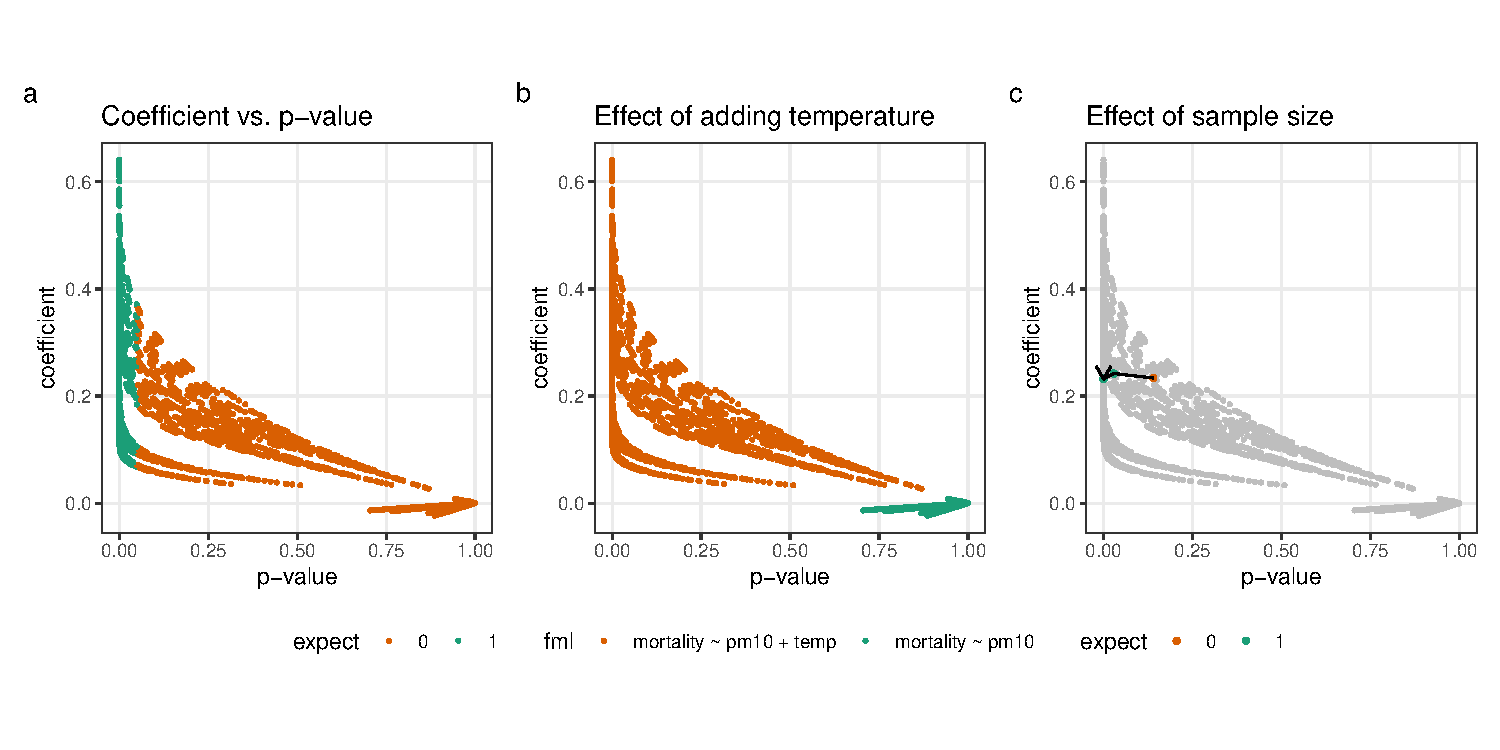
\includegraphics{index_files/figure-pdf/fig-result-universe-1.pdf}

}

\caption{\label{fig-result-universe}The result universe of linear
regression model to study the effect of PM10 on mortality: a) colored by
whether the p-value of PM10is significant (less than 0.05), b) the
effect of adding temperature to the model for a sample size of 500, c)
the effect of increasing sample size for a fixed correlation structure.}

\end{figure}%

\textsubscript{Source:
\href{https://huizezhang-sherry.github.io/paper-analysis-plan/index.qmd.html}{Article
Notebook}}

\section{Discussion}\label{discussion}

\begin{itemize}
\item
  how to systematically simulate data is still unknown, sensitivity of
  the simulation to the results
\item
  plotting is a critical way to check data and they can still be frame
  into a unit test. it is a open problem to how to encode the
  visualization into the unit tests. Maybe a procedure like confirm plot
  (this looks alright to you) and then press the button to continue
\item
  currently no automated way to generate unit tests
\end{itemize}

\section{Conclusion}\label{sec-conclusion}


\renewcommand\refname{References}
  \bibliography{references.bib}



\end{document}
